
\section{Research Background} \label{sec:related}

TBD.

\subsection{Concurrency Bugs and Attacks in Multithreaded Programs} \label{sec:others-work}

% P1: multithreading, hard to get right, plagued with concurrency bugs.
P1: TBD.

\begin{figure}[t]
\centering
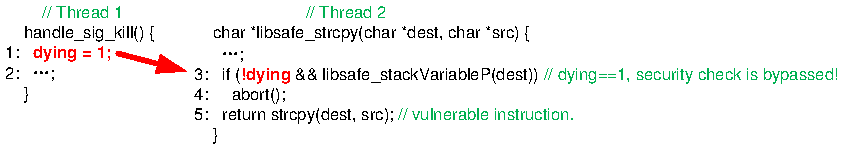
\includegraphics[width=0.99\columnwidth]{figures/libsafe}
\vspace{-.05in}
\caption{{A concurrency attack in libsafe.}} \label{fig:libsafe}
\vspace{-.05in}
\end{figure}

% P2: Can lead to various exploits. Mention our initial study, types of software, 
% and types of concurrency exploits. Just like bugs in single threaded program 
% leader to exploits, concurrency bugs can lead to concurrency attacks.
% Mention HotPart, found XX exploits. We: found YY exploits. patterns.
% Two examples.
P2: TBD.

% \subsubsection{Priliminary Study on Real-world Concucrency Attacks} 
% \label{sec:model-result}


% P3: A key reason: a program can run into too many thread interleavings at runtime.
% Hard to make sure all thread intleravings are correct. Mention our previous 
% work Parrot, exponentially many.
P3: TBD.

% P4: Then, challenges come: a concurrency 
% attack model should incorporate thread interleavings. A detection methond 
% should also consider the consequence of thread interleavings. A runtim 
% technique must think of ways to replicate and reduce the amount thread interleavings.
P4: TBD.


\subsection{Related Work by Others} \label{sec:others-work}

\para{Concurrency reliability techniques.} TBD. Emphasis that these tools are 
complementary with \xxx because \xxx focuses on the security consequence of bugs.
Detection tools.
Debugging tools.
Avoidance/fixing tools.
Also mention concurrency attacks (HotPar).

\para{TOCTTOU attacks.} TBD. Concurrency attacks are serious than normal TOCTTOU.

\para{Traditional security defense techniques.} TBD.
Mention shadow memory approaches.
Mention security libraries.
Mention stack overflow detection.
Say these are mainly for single-threaded programs.

\para{State machine replication.} TBD.
Say systems.
Also say checkpoint restore techniques.

\para{DMT systems.} TBD.



\subsection{Related Work by the PI} \label{sec:my-work}

First emphasis debugging experience on concurrency. Program analysis.
Then mention security exploits found in Woodpecker.
Then mention runtime systems.

A key requirement to making SMR practically support multi-threading is that all 
replicas must run the same thread interleavings so that the replica executions 
won't diverge. \smt~\cite{smt:cacm}, an advanced reliable multi-threading 
runtime technique invented by my collaborators and me, meets this requirement. 
This is because \smt can greatly reduce the number of possible thread 
interleavings in multi-threaded programs for all inputs with low performance 
overhead, making replications of multi-threaded programs almost as easy as 
single-threaded ones. In the last four years, the PI has been collaborating 
with Columbia and CMU researchers to build three \smt systems, 
\tern~\cite{cui:tern:osdi10}, \peregrine~\cite{peregrine:sosp11}, and 
\parrot~\cite{parrot:sosp13}, with each addressing distinct research 
challenges. Notably, \parrot, our latest system, is the first \smt runtime 
system that is fast (12.7\% mean overhead for all evaluated programs) on a wide 
range of 100+ popular multi-threaded programs. We have 
put all \parrot's source code and raw evaluation results on 
\url{http://github.com/columbia/smt-mc} for future research and industrial 
deployments. Due to \parrot's high practicality, we plan to leverage it in this 
proposed \msmr system.

To show \smt's potential, we have applied these systems to greatly improving 
software reliability and security, including improving precision and simplicity 
of program analysis and verification~\cite{wu:pldi12}, making debugging 
concurrency errors much easier~\cite{cui:tern:osdi10}, and improving coverage 
of model checking~\cite{parrot:sosp13}. Our work have also been leveraged by 
the community: some techniques in our \tern system~\cite{cui:tern:osdi10} has 
been used by University of Washington Seatle researchers on computing a small 
set of thread interleavings covering all inputs~\cite{ics:oopsla13}, and our 
\parrot runtime system has been integrated with a CMU software model 
checker~\cite{dbug:spin11}.

Our experience on building \smt runtime sytems can address the two 
aforementioned major research challanges of the \smt and SMR integration. In 
addition, our techniques on program analysis, verification, and model checking 
can be deployed in \msmr replicas and enhance their reliability and security.


